%-------------------------------------------------------------------------------
% Methoden
%-------------------------------------------------------------------------------
\section{Ergebnisse}
Nachfolgend erfolgt die Untersuchung der Ergebnisse des Experiments.

\subsection{Beschreibung der Stichprobe}\label{beschreibung}
Die Studie startete am 05.07.2020 und endete am 07.09.2020. Das Experiment war für die Dauer der Studie durchgehend erreichbar. Insgesamt nahmen 221 Teilnehmer an dem Experiment teil. Davon haben 17 Personen das Experiment vollständig durchlaufen und sämtliche Fragen korrekt beantwortet. Aus dem Datensatz wurden zunächst 9 Einträge entfernt, die nicht in der Auswertung berücksichtigt werden. Bei diesen Einträgen handelte es sich um Mehrfachteilnahmen, die sich durch eine identische IP-Adresse sowie identische User-Agents auszeichneten. Es wurde in diesem Fall lediglich die erstmalige Teilnahme berücksichtigt. Damit hat der bereinigte Datensatz einen Umfang von 212 Teilnehmern.

Von den verbleibenden Versuchspersonen gaben 77.7\% der Teilnehmer an, männlich zu sein. 12.8\% gaben ein weibliches Geschlecht und 9.5\% ein anderes Geschlecht an. Der Großteil der Teilnehmer gab an, über gute (43.4\%) oder sehr gute (42.0\%) Englischkenntnisse zu verfügen. Lediglich 9.0\% verfügten über schlechte Kenntnisse und nur 5.7\% verfügten über keinerlei englische Sprachkenntnisse. Die Altersverteilung der Versuchspersonen ist wie folgt: 39.6\% gaben 18-29 Jahre an, 33.0\%  29-39 Jahre,  15.1\% 39-59 Jahre, 6.6\% weniger als 18 Jahre und 5.7\% gaben an, älter als 59 Jahre zu sein. Damit waren zum Zeitpunkt des Experiments 87.7\% der Teilnehmer zwischen 18 und 59 Jahre alt. Davon nutzt ein Großteil die Kommandozeile mindestens einmal im Monat (42.9\% täglich, 24.5\% wöchentlich, 10.4\% monatlich). Demgegenüber nutzen 13.2\% die Kommandozeile selten (1x im Jahr oder weniger) oder gar nicht (10.4\%). Damit setzt sich die Stichprobe aus überwiegend jungen Versuchspersonen, die über gute Englischkenntnisse verfügen und bereits erste Erfahrungen mit der Kommandozeile haben, zusammen.

\subsection{Deskriptive Statistik}

\begin{figure}[htbp]
    \centering
    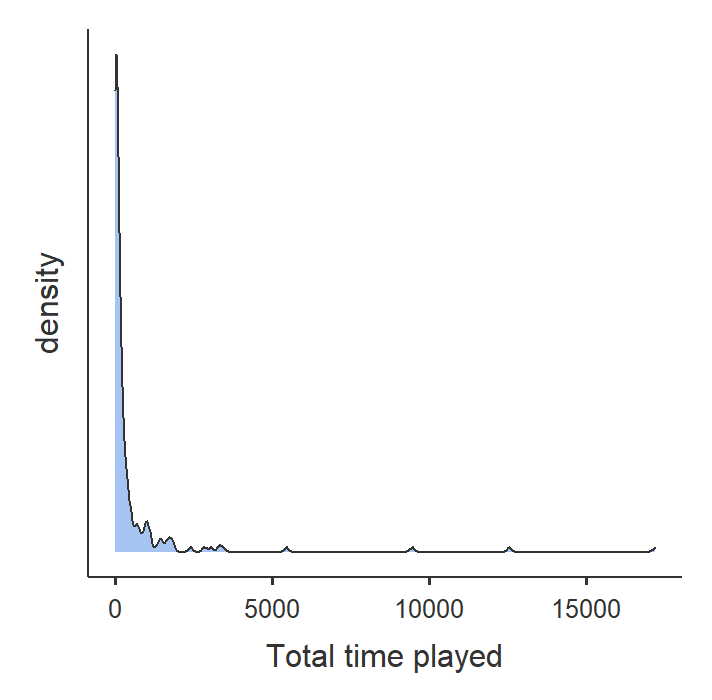
\includegraphics[width=0.5\textwidth]{img/auswertung/density.png}
    \caption{Die Verteilungskurve aller Teilnehmer hinsichtlich der Gesamtspielzeit.}
    \label{density}
\end{figure}

Im Mittel verbrachten die Teilnehmer 8 Minuten und 33 Sekunden (SD= 28.18 Minuten) mit dem Experiment und setzten dabei im Mittel 16.2 Befehle ab (SD= 22.0). Sowohl bei der Gesamtdauer als auch bei der Anzahl der abgesendeten Befehle gibt es extreme Ausreißer nach oben. So investierte ein Teilnehmer fast 5 Stunden in das Experiment und verwendete dabei 84 unterschiedliche Befehle. Diese enorme Streuung nach oben wird auch in Abbildung \ref{density} deutlich. Aus diesem Grund werden im Folgenden nicht nur die Mittelwerte sondern jeweils auch der Median betrachtet, da dieser robuster gegenüber Ausreißern ist.

% Anzahl Befehle
\begin{figure}[htbp]
    \centering
    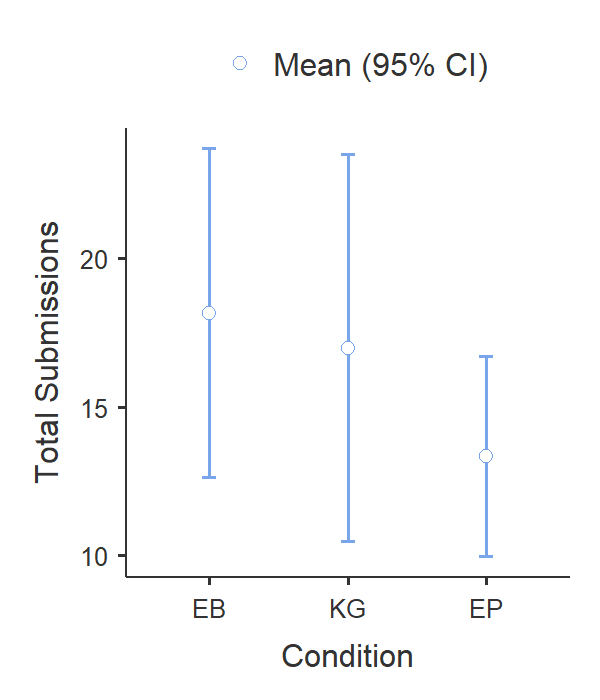
\includegraphics[width=0.5\textwidth]{img/auswertung/mean_total_subs.png}
    \caption{Mittelwerte für die Gesamtzahl abgesetzter Befehle. EB= Experimentalbedingung Abzeichen, KG= Kontrollgruppe und EP = Experimentalbedingung Fortschrittsanzeige.}
    \label{mean_subs}
\end{figure}
Die mittlere Anzahl abgesetzter Befehle ist der in der Versuchsbedingung 'Abzeichen' mit 18.2 (SD = 24.6) am höchsten. Die Kontrollgruppe weist im Vergleich eine mittlere Anzahl abgesetzter Befehle von 17.0 (SD = 25.7) auf. Auffällig ist, dass Teilnehmer der Versuchsbedingung 'Fortschrittsanzeige' im Mittel lediglich 13.1 (SD = 14.4) Befehle absetzten und damit deutlich weniger als die anderen Versuchsbedingungen. Die Mittelwerte sind in Abbildung \ref{mean_subs} dargestellt. Hier fällt erneut das breite Streuungsintervall auf. Betrachtet man entsprechend den Median, fallen die Ergebnisse anders aus. So weist die Versuchsbedingung 'Abzeichen' mit 8.5 erneut die höchste Anzahl abgeschickter Befehle auf. Allerdings bleibt die Experimentalbedingung Fortschrittsanzeige (8.0 Befehle) in diesem Fall oberhalb der Kontrollgruppe (7.0 Befehle). Der Median der erfolgreich gelösten Aufgaben ist bei allen drei Gruppen mit 3.0 gelösten Aufgaben identisch. 

% Investierte Zeit
\begin{figure}[htbp]
    \centering
    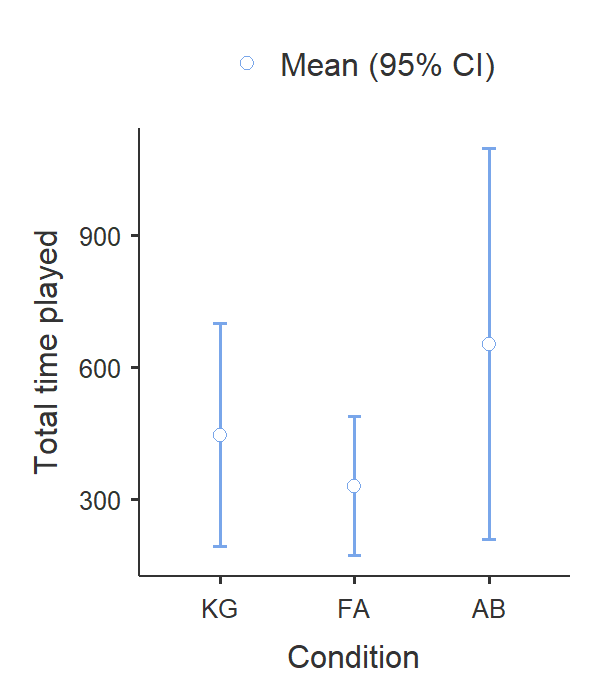
\includegraphics[width=0.5\textwidth]{img/auswertung/mean_time.png}
    \caption{Mittelwerte für die Gesamtzeit, die die Teilnehmer in das Experiment investierten. EB= Experimentalbedingung Abzeichen, KG= Kontrollgruppe und EP = Experimentalbedingung Fortschrittsanzeige.}
    \label{mean_time}
\end{figure}
Betrachtet man die Zeit, die die Teilnehmer im Mittel in das Experiment investiert haben, fällt auf, dass die Teilnehmer der Versuchsbedingung 'Abzeichen' mit 733 Sekunden (~12 Minuten, SD= 2414 Sekunden) wesentlich mehr Zeit als die der Kontrollgruppe mit 485 Sekunden (~8 Minuten, SD= 1316 Sekunden) aufgebracht haben. Letztere haben wiederum deutlich mehr Zeit investiert, als die Probanden der Versuchsbedingung 'Fortschrittsanzeige'. Diese brachten es auf vergleichsweise kurze 302 Sekunden (~5 Minuten, SD= 768 Sekunden). Die entsprechenden Mittelwerte sind in Abbildung \ref{mean_time} dargestellt. Betrachtet man auch hier den Median und nicht die Mittelwerte, ändert sich das Ergebnis. Die Probanden der Experimentalbedinungen investierten im Median mehr Zeit als die Kontrollgruppe. So bringen es Teilnehmer der Bedingung 'Abzeichen' auf 105 Sekunden (~2 Minuten) und bringen damit ähnlich viel Zeit für das Experiment wie die Probanden der Bedingung 'Fortschrittsanzeige' (107 Sekunden) auf. In der Kontrollgruppe ist der Median hingegen 69 Sekunden.

Sowohl die investierte Gesamtzeit als auch die Anzahl abgesetzter Befehle zeichnen sich damit durch eine hohe Streuung aus. Betrachtet man jeweils den Median weisen beide Experimentalbedingung eine messbare Erhöhung in der Gesamtzeit und der Befehlszahl gegenüber der Kontrollgruppe auf. Aufgrund der hohen Diskrepanz zwischen Median und Mittelwert sowie der extrem hohen Standardabweichung habe ich beschlossen extreme Ausreißer aus der weiteren Betrachtung auszuschließen. Bei diesen Ausreißern gehe ich davon aus, dass eine, von den Spielelementen unabhängige, Intrinsische Motivation vorliegt. Als Grenzwert wählte ich $\pm 2\sigma$. Dies führt dazu, dass sämtliche Teilnehmer mit mehr als 3896 Sekunden Spieldauer aus dem Datensatz ausgeschlossen werden. Zusätzlich werden nur Teilnehmer berücksichtigt, die mindestens einen Befehl abgesetzt haben. Damit reduziert sich der Datensatz im folgenden auf einen Umfang von 190.

\subsection{Hypothesenüberprüfung}
Die aufgestellten Hypothesen werden durch einen t-Test und eine einfaktorielle  ANOVA  Varianzanalyse überprüft. Zunächst sind die Voraussetzungen Normalverteilung und Varianzhomogenität zu prüfen. Da jede Versuchsbedingung einen Umfang von deutlich über 30 Probanden aufweist, kann von einer Normalverteilung ausgegangen werden. Um die Vorraussetzung der Varianzhomogenität zu prüfen, habe ich einen Levene-Test durchgeführt. Bei diesem handelt es sich um einen Signifikanztest. Dieser prüft, ob die Varianzen innerhalb von zwei oder mehr Grundgesamtheiten (Gruppen) gleich sind (H0). Daraus ergibt sich die Alternativhypothese (H1), dass mindestens ein Gruppenpaar ungleiche Varianzen besitzt. Befindet sich der p-Wert unterhalb  eines zuvor definierten Signifikanzniveaus sind die Unterschiede in den Varianzen der unterschiedlichen Stichproben signifikant. Folglich kann die Nullhypothese des Tests abgelehnt werden. 
\begin{table}[htbp]
\centering
\begin{tabular}{ |p{2.6cm}||p{2.0cm}|p{2.0cm}|p{2.0cm}|p{2.0cm}| }
 \hline
 \multicolumn{5}{|c|}{Test auf Varianzhomogenität (Levene's)} \\
 \hline
 & F & df1 &df2 &p \\
 \hline
  Befehlanzahl   & 1.55    & 2 &   187 & 0.215\\
  Gesamtspielzeit   & 3.09    & 2 &   187 & 0.048\\
 \hline
\end{tabular}
\caption{Levene-Test auf Varianzhomogenität für die Bedingungen Befehlsanzahl und Gesamtspielzeit.}
\label{levene}
\end{table}
Für den Test gehe ich von einem Signifikanzniveau von 5\% aus. Wie in Tabelle \ref{levene} zu sehen, ist der Levene-Test nur für die Gesamtspielzeit unterhalb des Signifikanzniveaus von 5\% und damit signifikant. Dies schließt jedoch die Verwendung eines t-Tests nicht aus, da dieser sehr robust gegenüber Verletzungen seiner Voraussetzungen ist. Somit kann ein t-Test für die Bewertung der Gesamtanzahl abgesetzter Befehle angewendet werden.

\paragraph{Hypothese 1}
Die Hypothese lautete: \textit{Probanden, die Abzeichen erhalten, verbringen im Mittel mehr Zeit mit dem Experiment als eine Kontrollgruppe ohne Fortschrittsanzeige.} Diese Hypothese konnte mit $t(124)=0.00332$, $p=.501$ nicht bestätigt werden. Der t-Test war ebenfalls nicht signifikant. Zusätzlich prüfte ich, ob Teilnehmer mehr Befehle absetzten und entsprechend aktiver waren, wenn diese ein Abzeichen erhielten. Auch diese Hypothese konnte mit $t(124)=0.167$, $p=.434$ nicht bestätigt werden.

\paragraph{Hypothese 2}
Die Hypothese lautete: \textit{Probanden, die eine Fortschrittsanzeige sehen, verbringen im Mittel mehr Zeit mit dem Experiment als eine Kontrollgruppe ohne Fortschrittsanzeige.} Diese Hypothese konnte mit $t(116)=1.21$, $p=.115$ nicht bestätigt werden, da der t-Test nicht signifikant war. Ergänzend prüfte ich erneut, ob Probanden der Experimentalbedingung 'Fortschrittsanzeige' mehr Fragen beantworteten als Probanden der Kontrollgruppe. Diese Hypothese konnte erneut nicht bestätigt werden, da der t-Test nicht signifikant war ($t(116)=0.745$, $p=.229$).
